\begin{frame}{Pad Detectors}

	\begin{figure}[h] 
		\centering
		\begin{subfigure}{0.45\textwidth}  
			\centering
			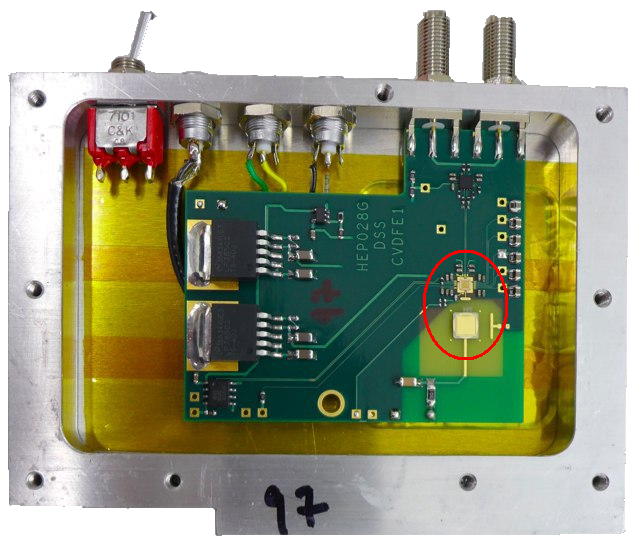
\includegraphics[height=0.45\textheight]{PadBox}
			\caption{fast amplifier box}
		\end{subfigure}
		\begin{subfigure}{0.45\textwidth} 
			\centering
			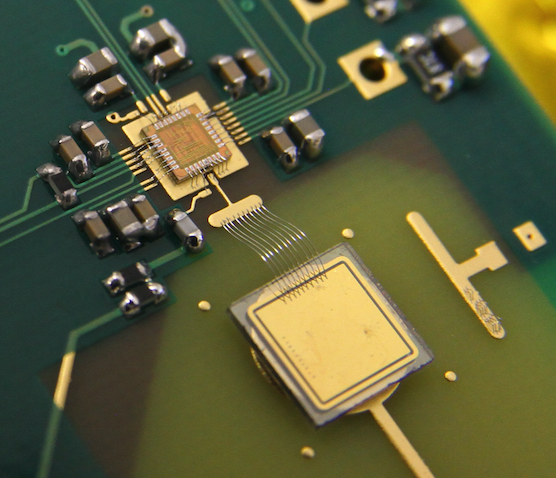
\includegraphics[height=0.45\textheight]{PadFull}
			\caption{diamond and fast amp} 	
		\end{subfigure} 
	\end{figure}
	
	\begin{itemize}
		\itemfill
		\item diamonds in custom built amplifier boxes from Ohio State University (OSU)
		\item cleaning, photo-lithography and Cr-Au metallisation at OSU
		\item low gain, fast amplifier with \orderof{\z{ns}} rise time
	\end{itemize}
	
\end{frame}
% ============================ FRAME 2 ==========================================>
\begin{frame}
	\frametitle{Waveforms}
	\vspace*{-20pt}
	\begin{center}
		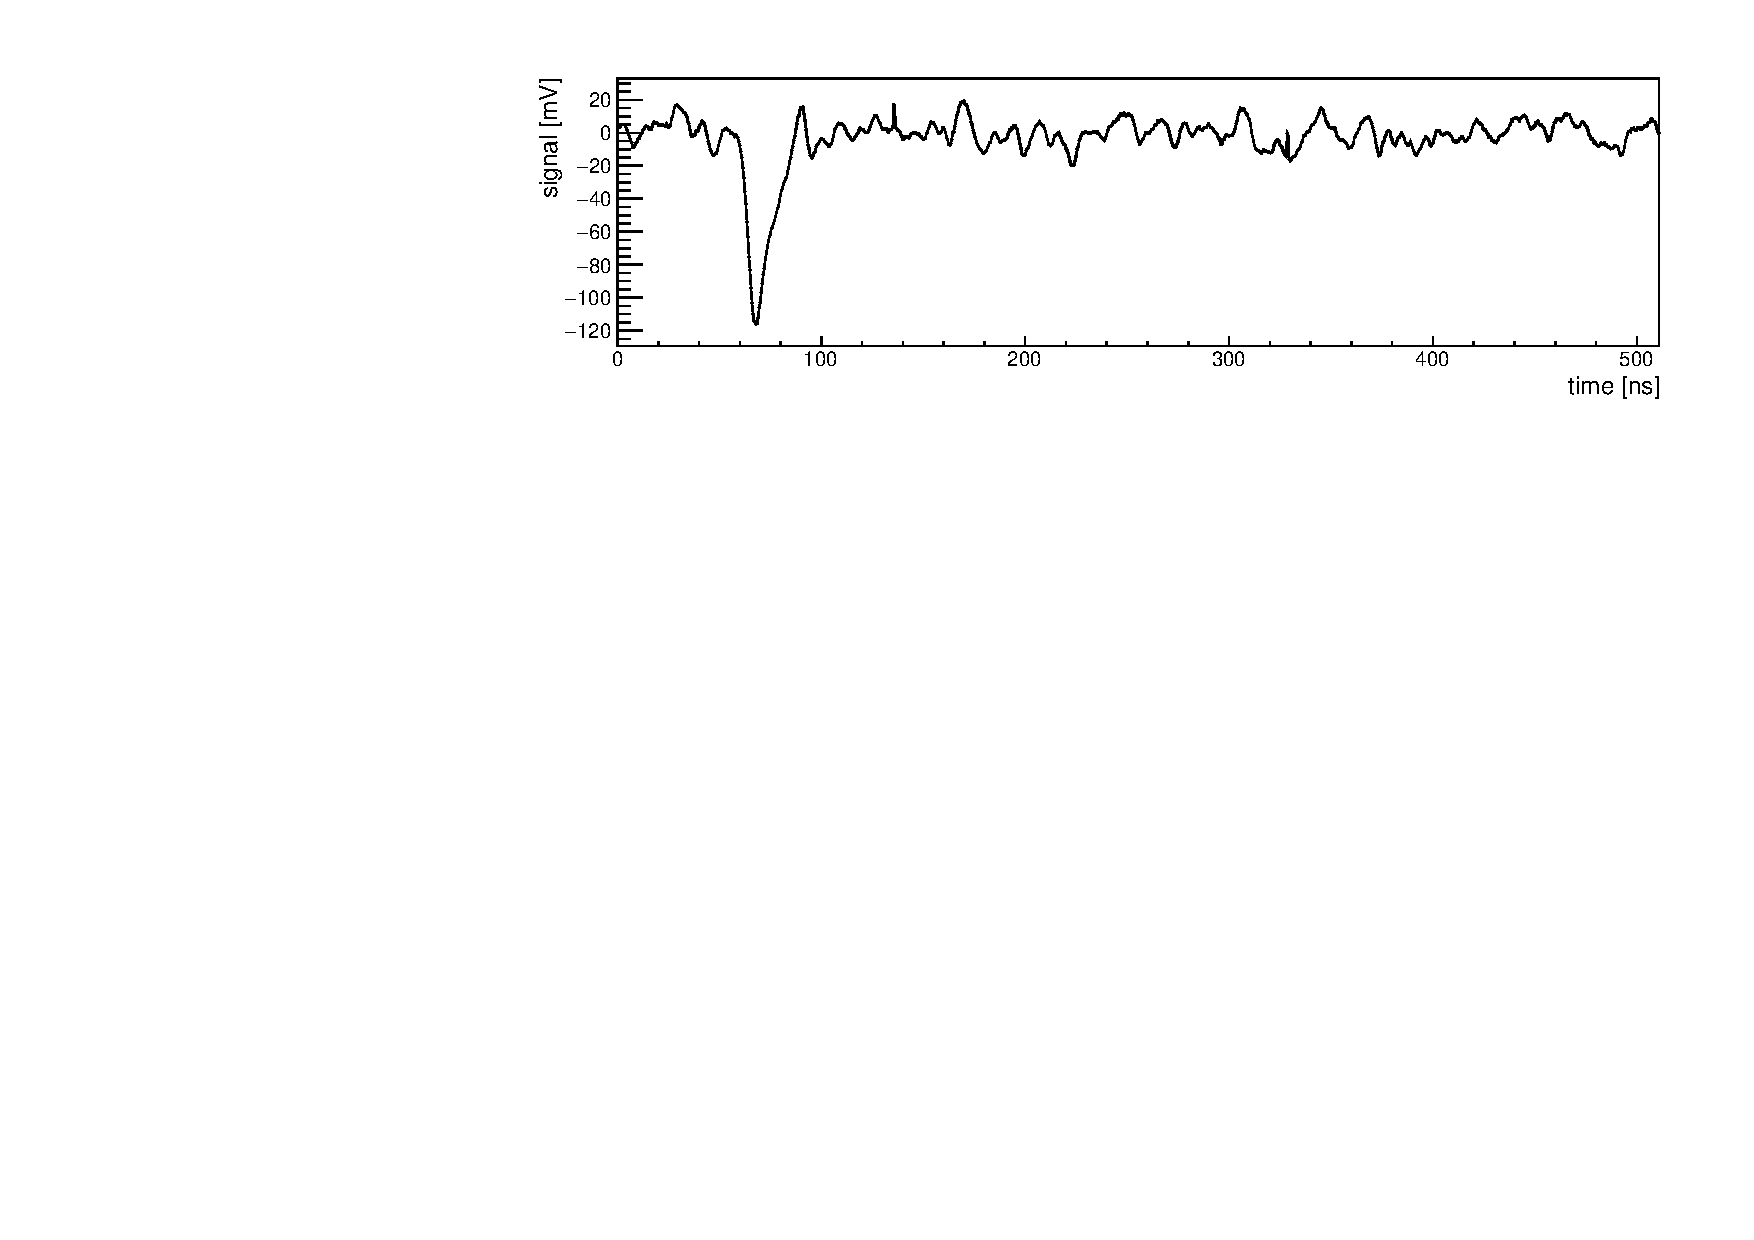
\includegraphics[angle=270, width=.7\textwidth]{SignalWaveform}\\
		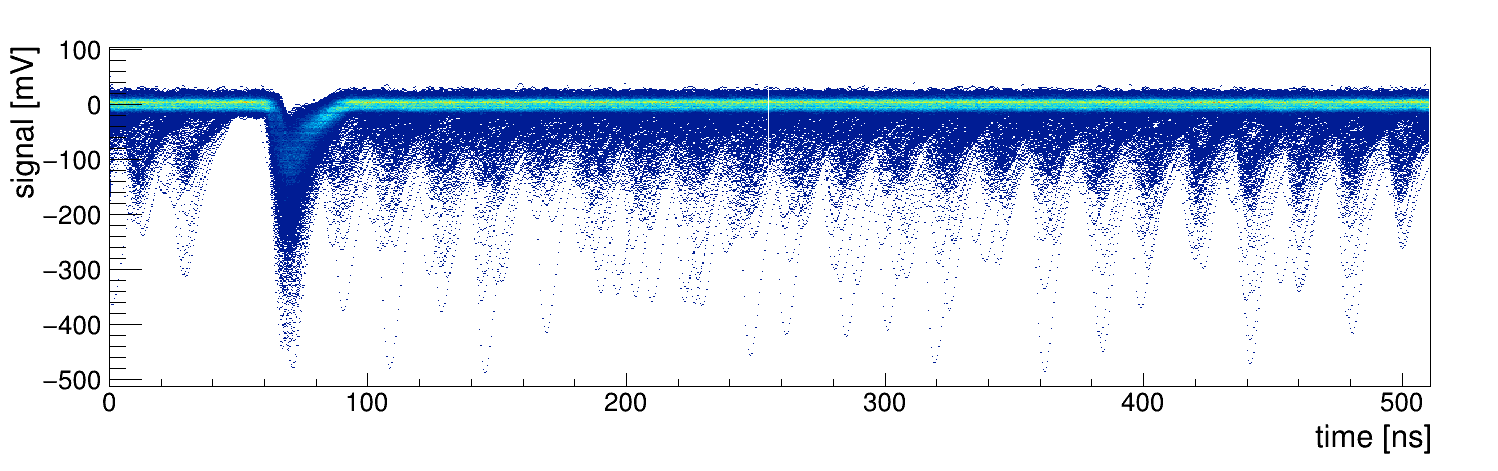
\includegraphics[width=.7\textwidth]{SignalWaveforms5000}
	\end{center}
	\begin{itemize}
		\item most frequented peak (\SI{\sim70}{ns}): triggered signal
		\item other peaks originate from other buckets ($\rightarrow$ resolve beam structure of \SI{\approx19.7}{ns})
		\item system does not allow signals in pre-signal bucket due to fastOR trigger deadtime
	\end{itemize}
\end{frame}
% ============================ FRAME 3 ==========================================>
\begin{frame}
	\frametitle{Pulse Height Calculation}
	\vspace*{-5pt}
	\begin{center}
		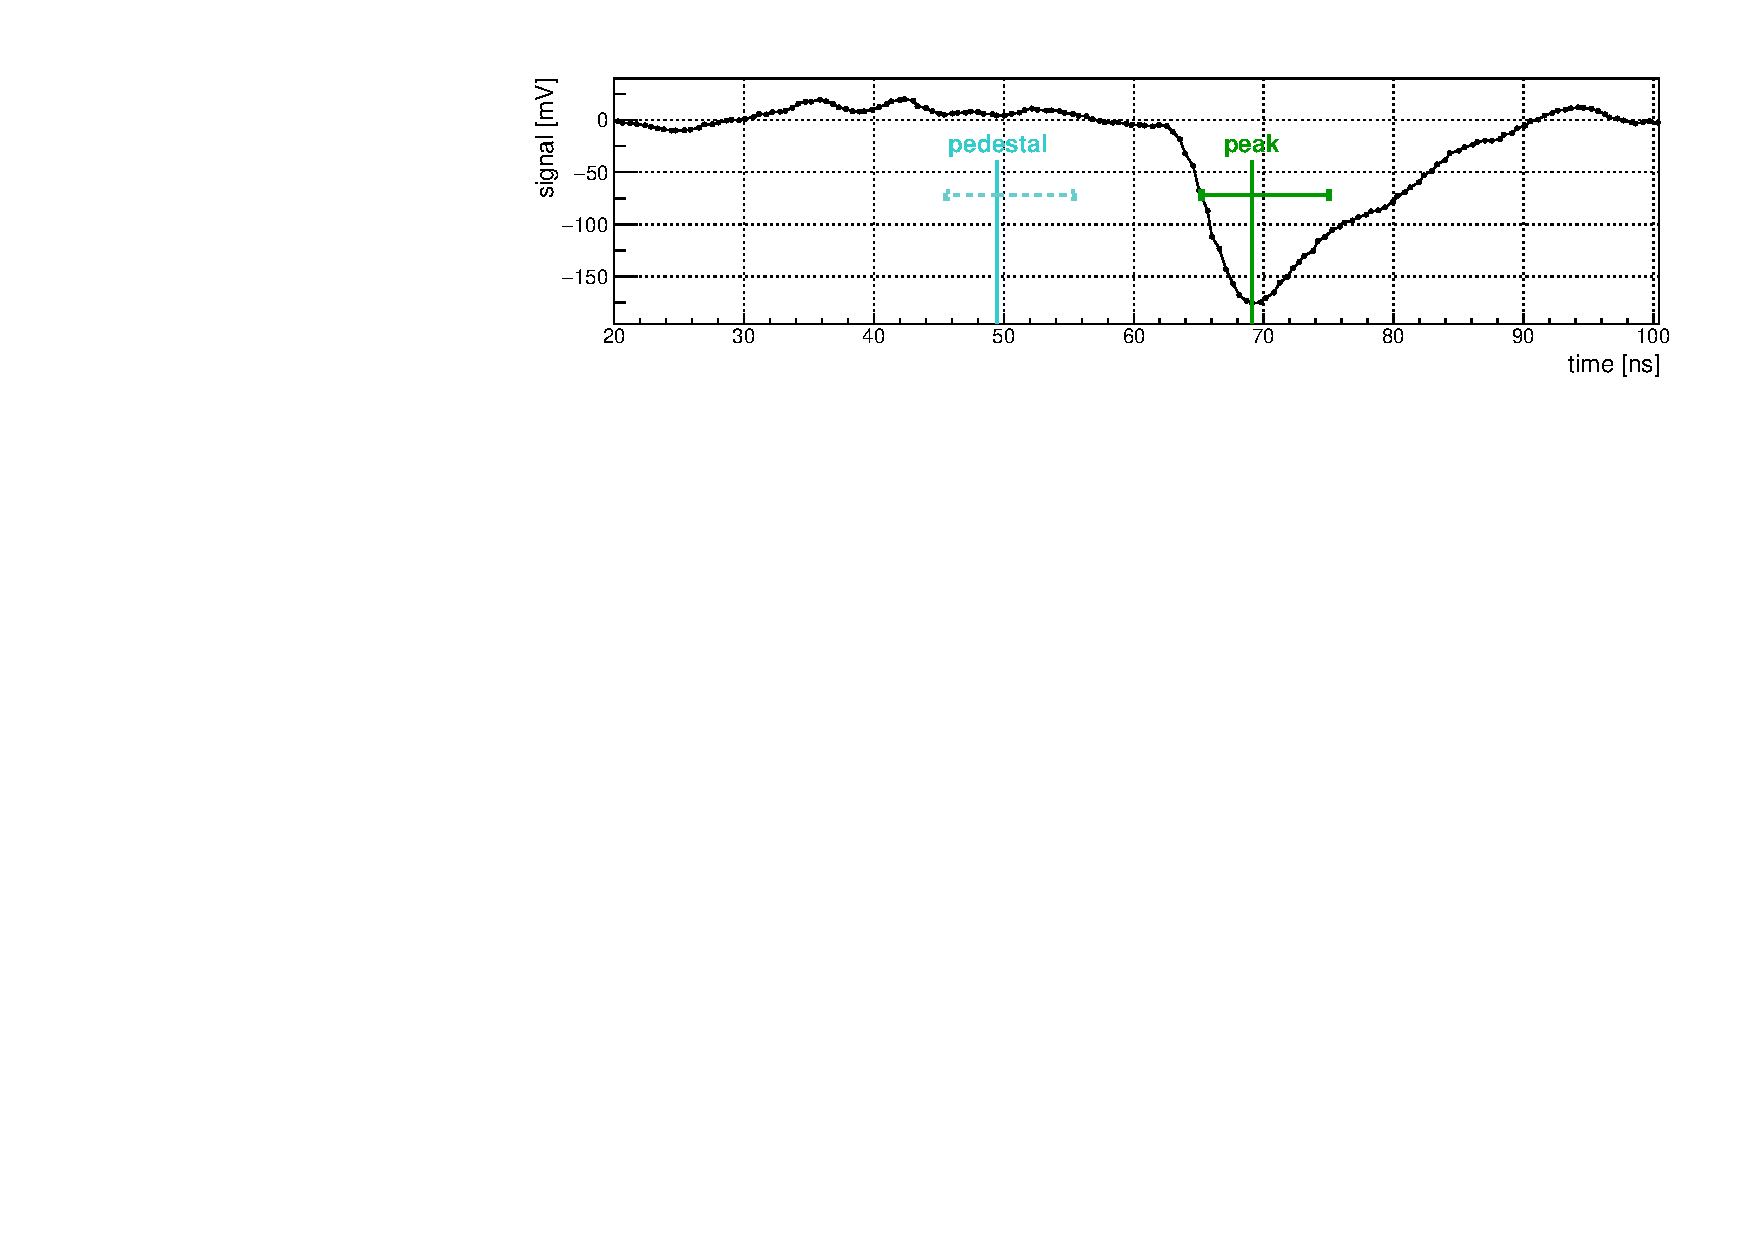
\includegraphics[angle=270, width=\textwidth]{intpeaks}\\
	\end{center}
	\vspace*{-5pt}
	\begin{itemize}
		\setlength{\itemsep}{\fill}
		\item finding the peak in the signal region
		\item integrating the signal in time fixed asymmetric integral around peak
		\item optimising the integral width by highest SNR (Integral / Pedestal Sigma)
	\end{itemize}
\end{frame}
% ============================ FRAME 4 ==========================================>
\begin{frame}
	\frametitle{Non-Irradiated Single Crystal Diamond}
	\def \sp {3.7cm}
	\begin{minipage}{\sp}
		\centering
		October 2015 
		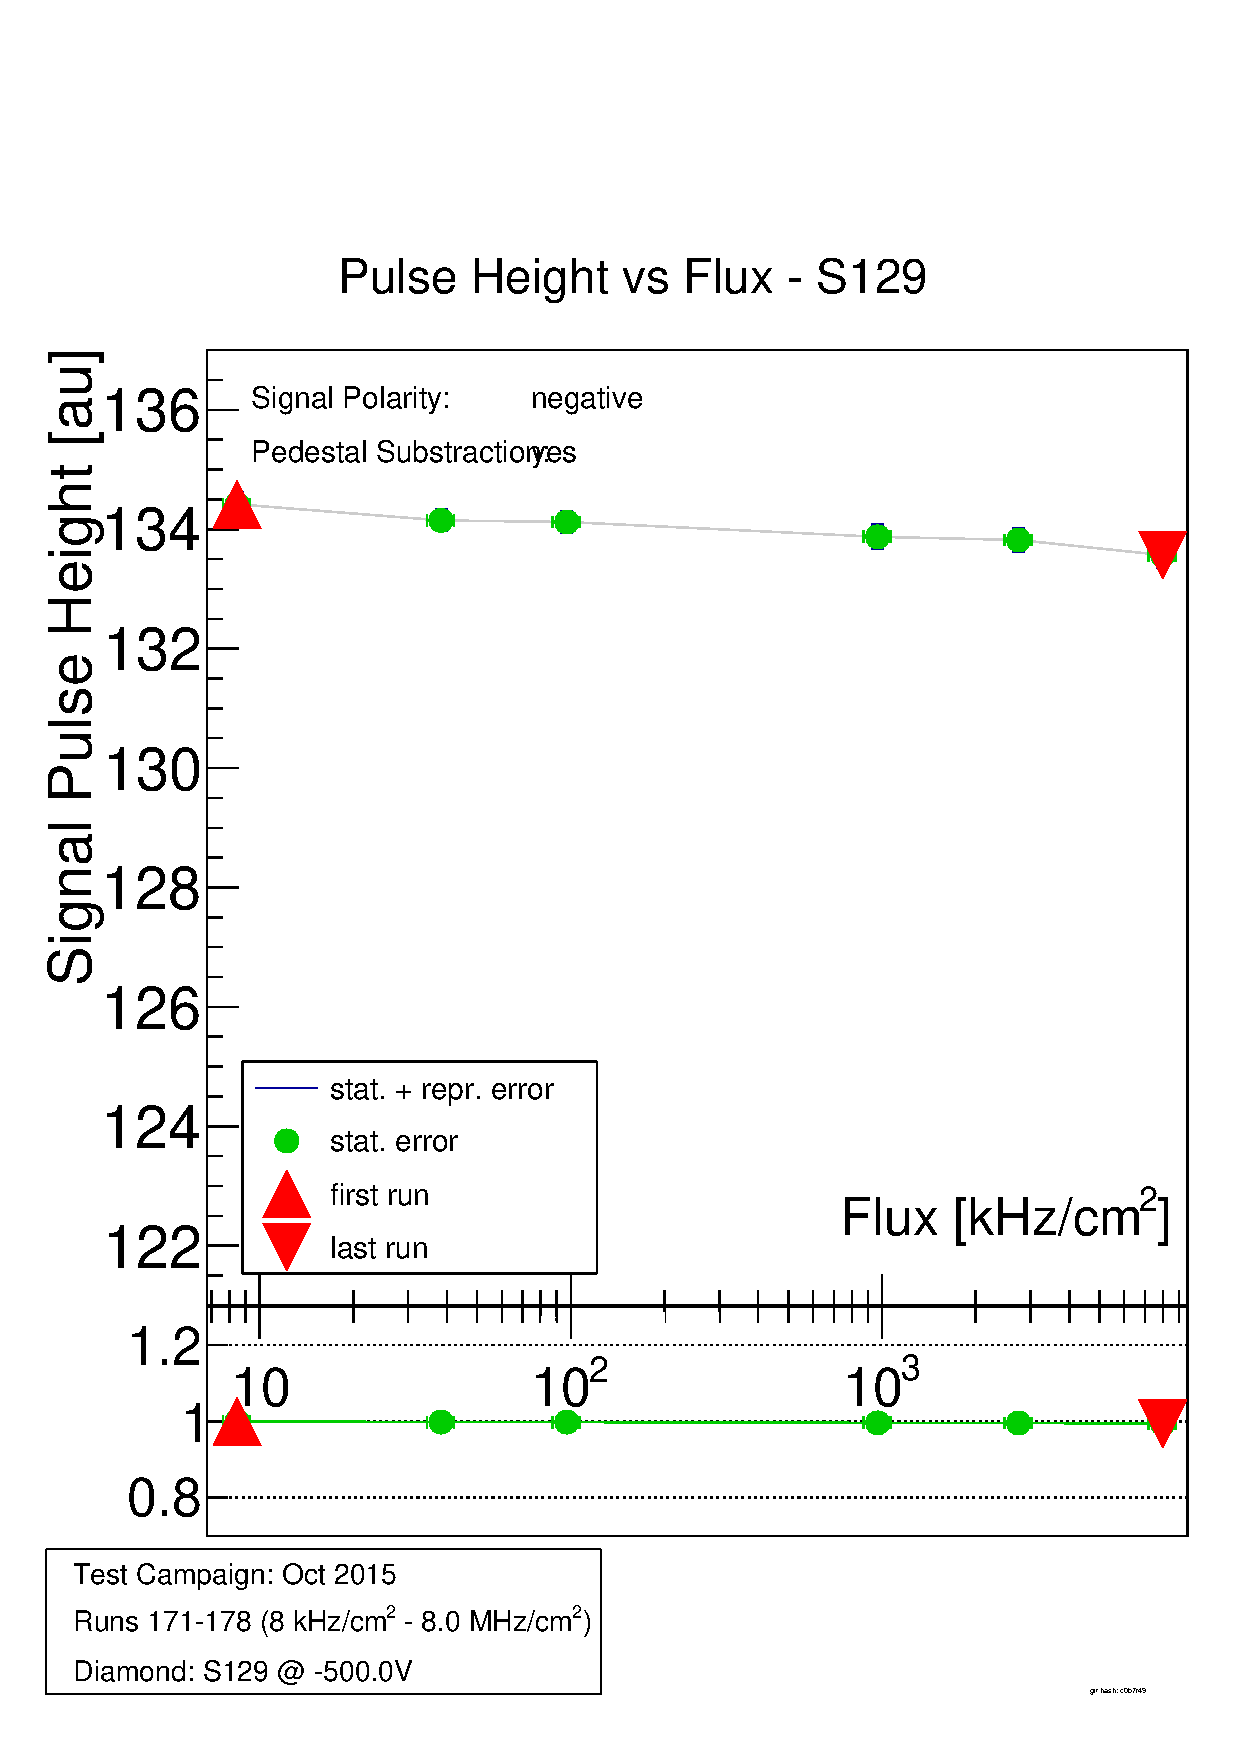
\includegraphics[width=\sp]{S129Oct15}\\
		noise $\upsigma\approx$ \SI{2.6}{au}
	\end{minipage}
	\hspace*{2pt}
	\begin{minipage}{\sp}
		\centering
		August 2016
		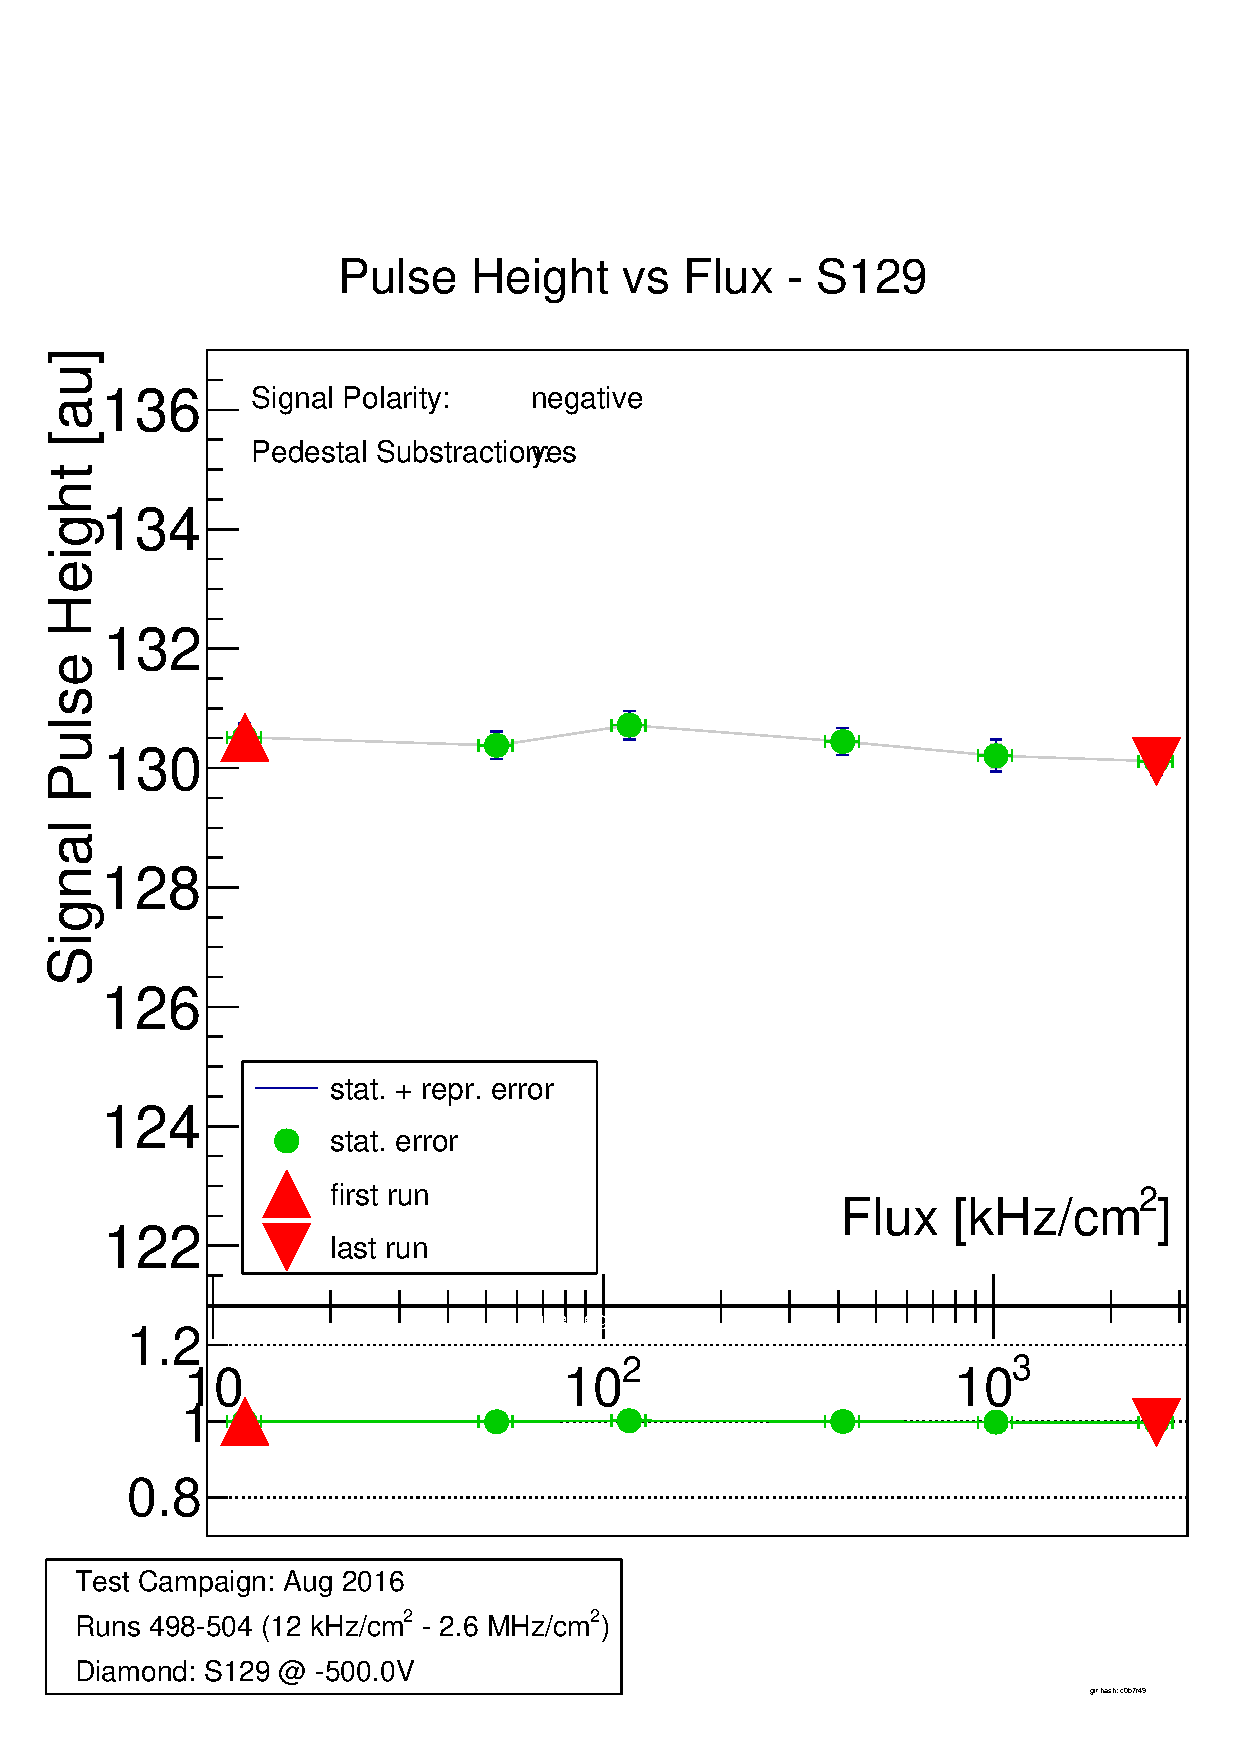
\includegraphics[width=\sp]{S129Aug16}\\
		noise $\upsigma\approx$ \SI{2.6}{au}
	\end{minipage}
	\hspace*{2pt}
	\begin{minipage}{\sp}
		\centering
		October 2016
		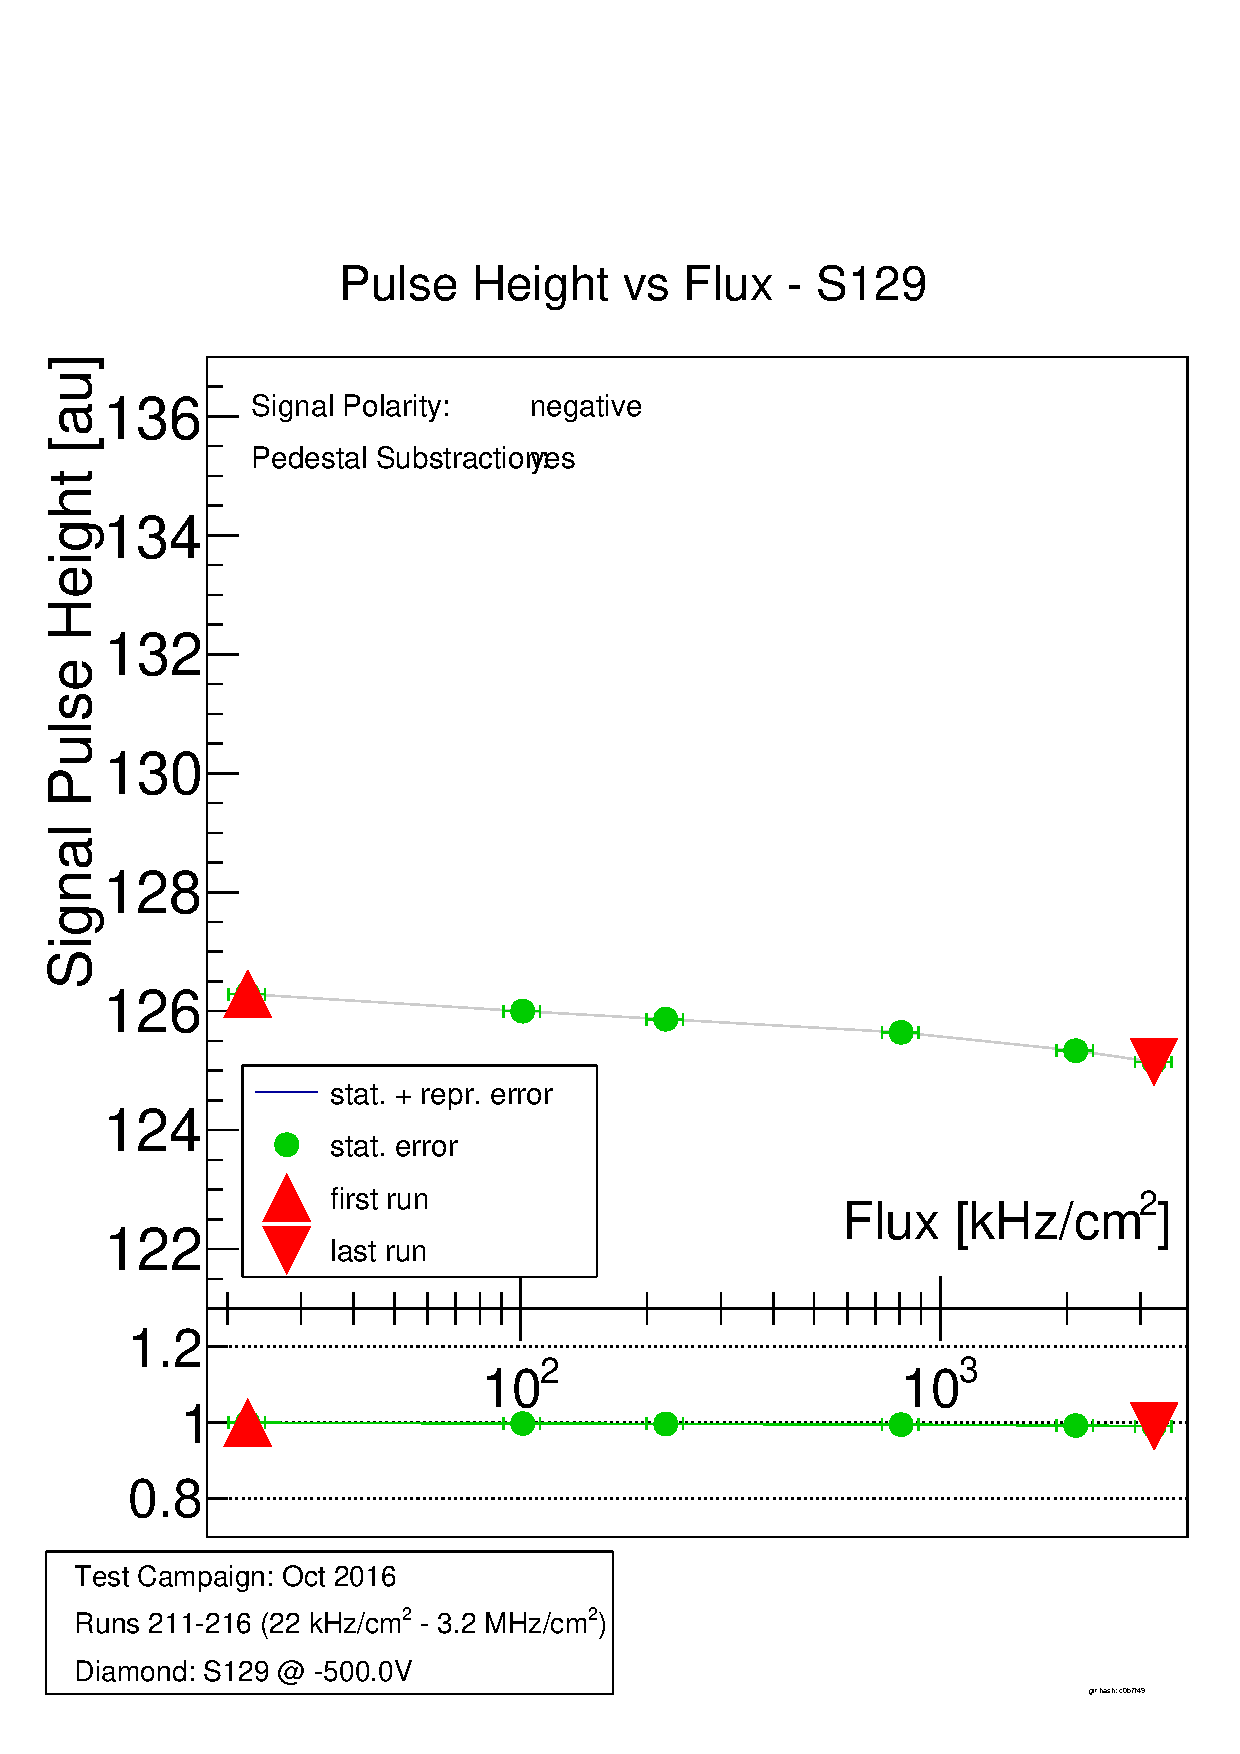
\includegraphics[width=\sp]{S129Oct16}\\
		noise $\upsigma \approx$ \SI{2.6}{au}
	\end{minipage}\s
	\begin{itemize}
		\item measurements taken under the same conditions
		\item noise stays the same
		\item pulse height very stable
	\end{itemize}
\end{frame}
% ============================ FRAME 5 ==========================================>
\begin{frame}
	\frametitle{Poly Crystal Diamond}
	\begin{minipage}{2.8cm}
		\centering
		August 2016 - \\unirradiated
		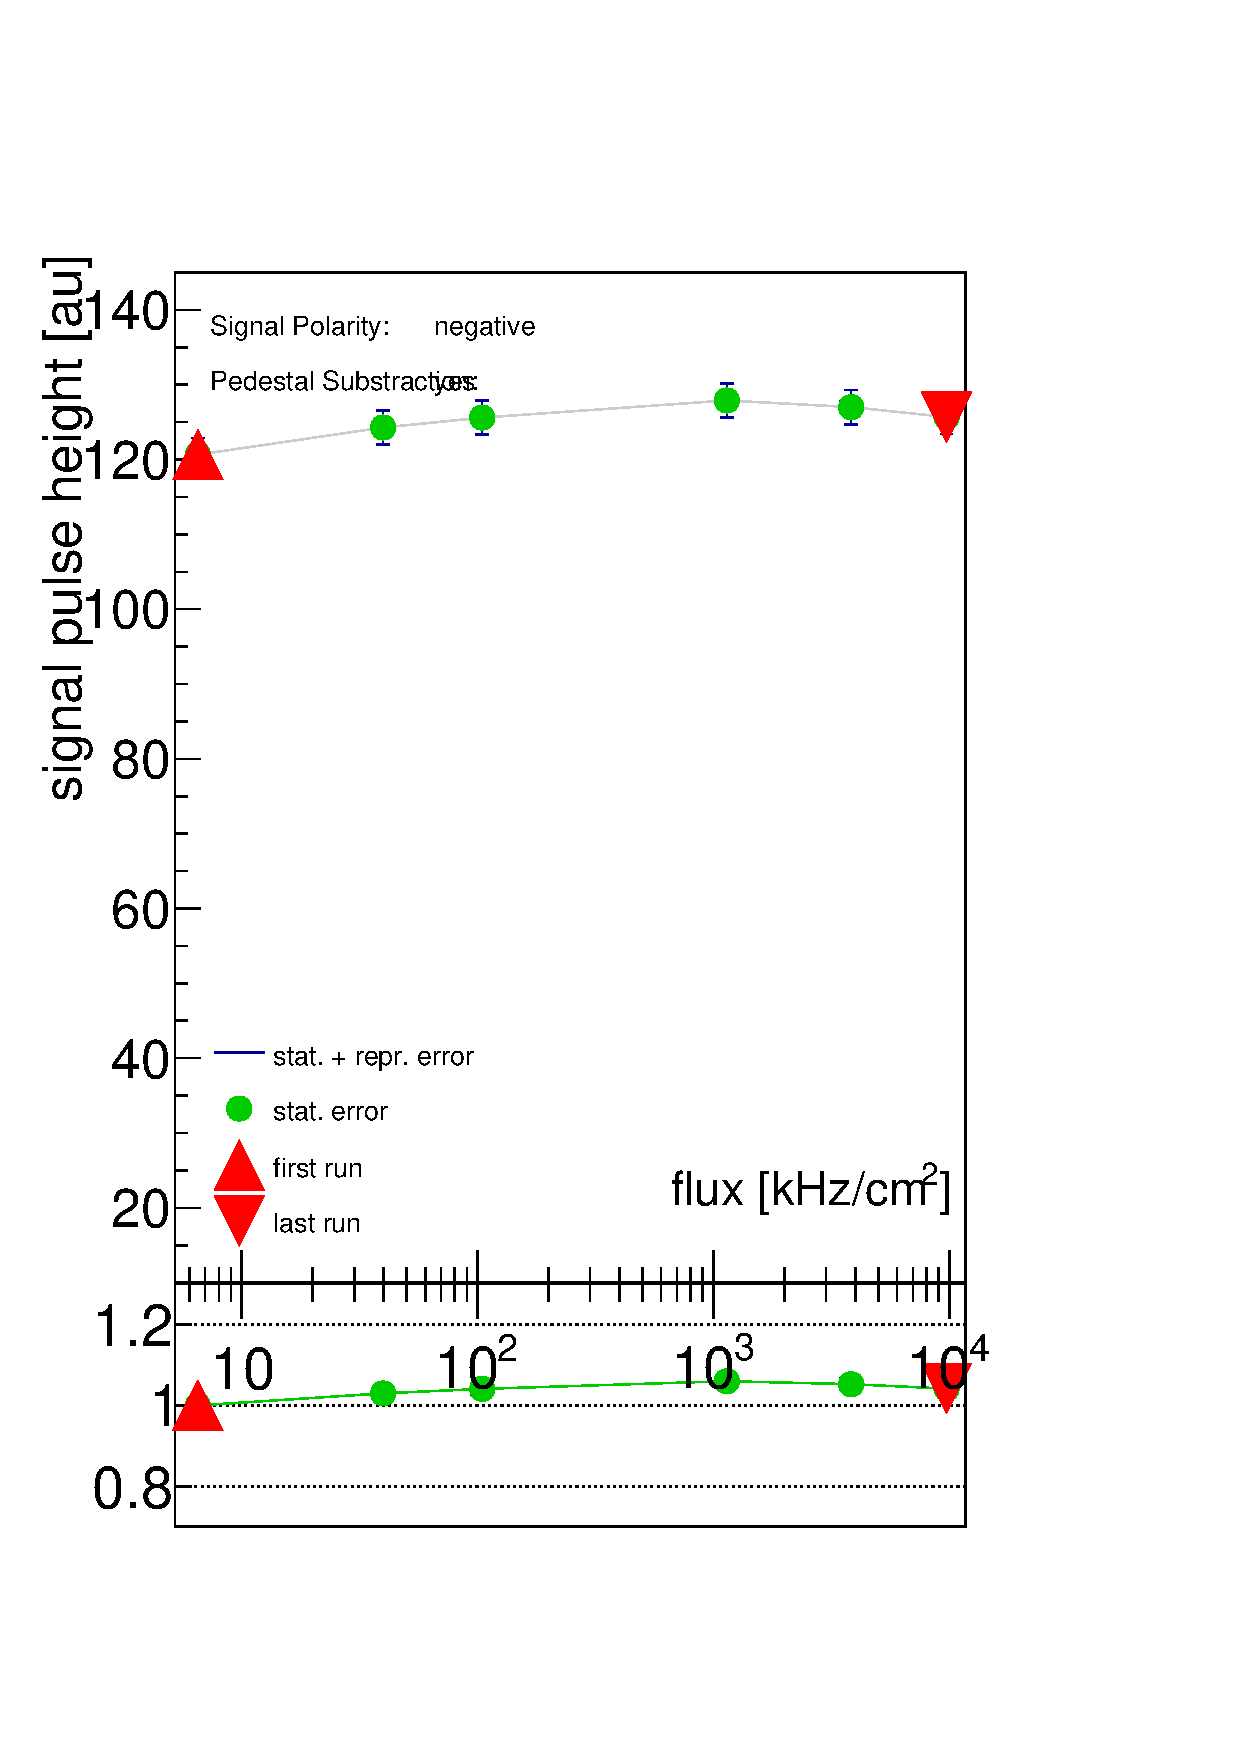
\includegraphics[width=3cm]{CPH1508_13_2.pdf}\\
		noise $\upsigma\approx$ \SI{4.9}{au}
	\end{minipage}
	\hspace*{2pt}
	\begin{minipage}{2.8cm}
		\centering
		October 2015 - \SI[exponent-product = \cdot]{5e14}{n/cm^{2}}
		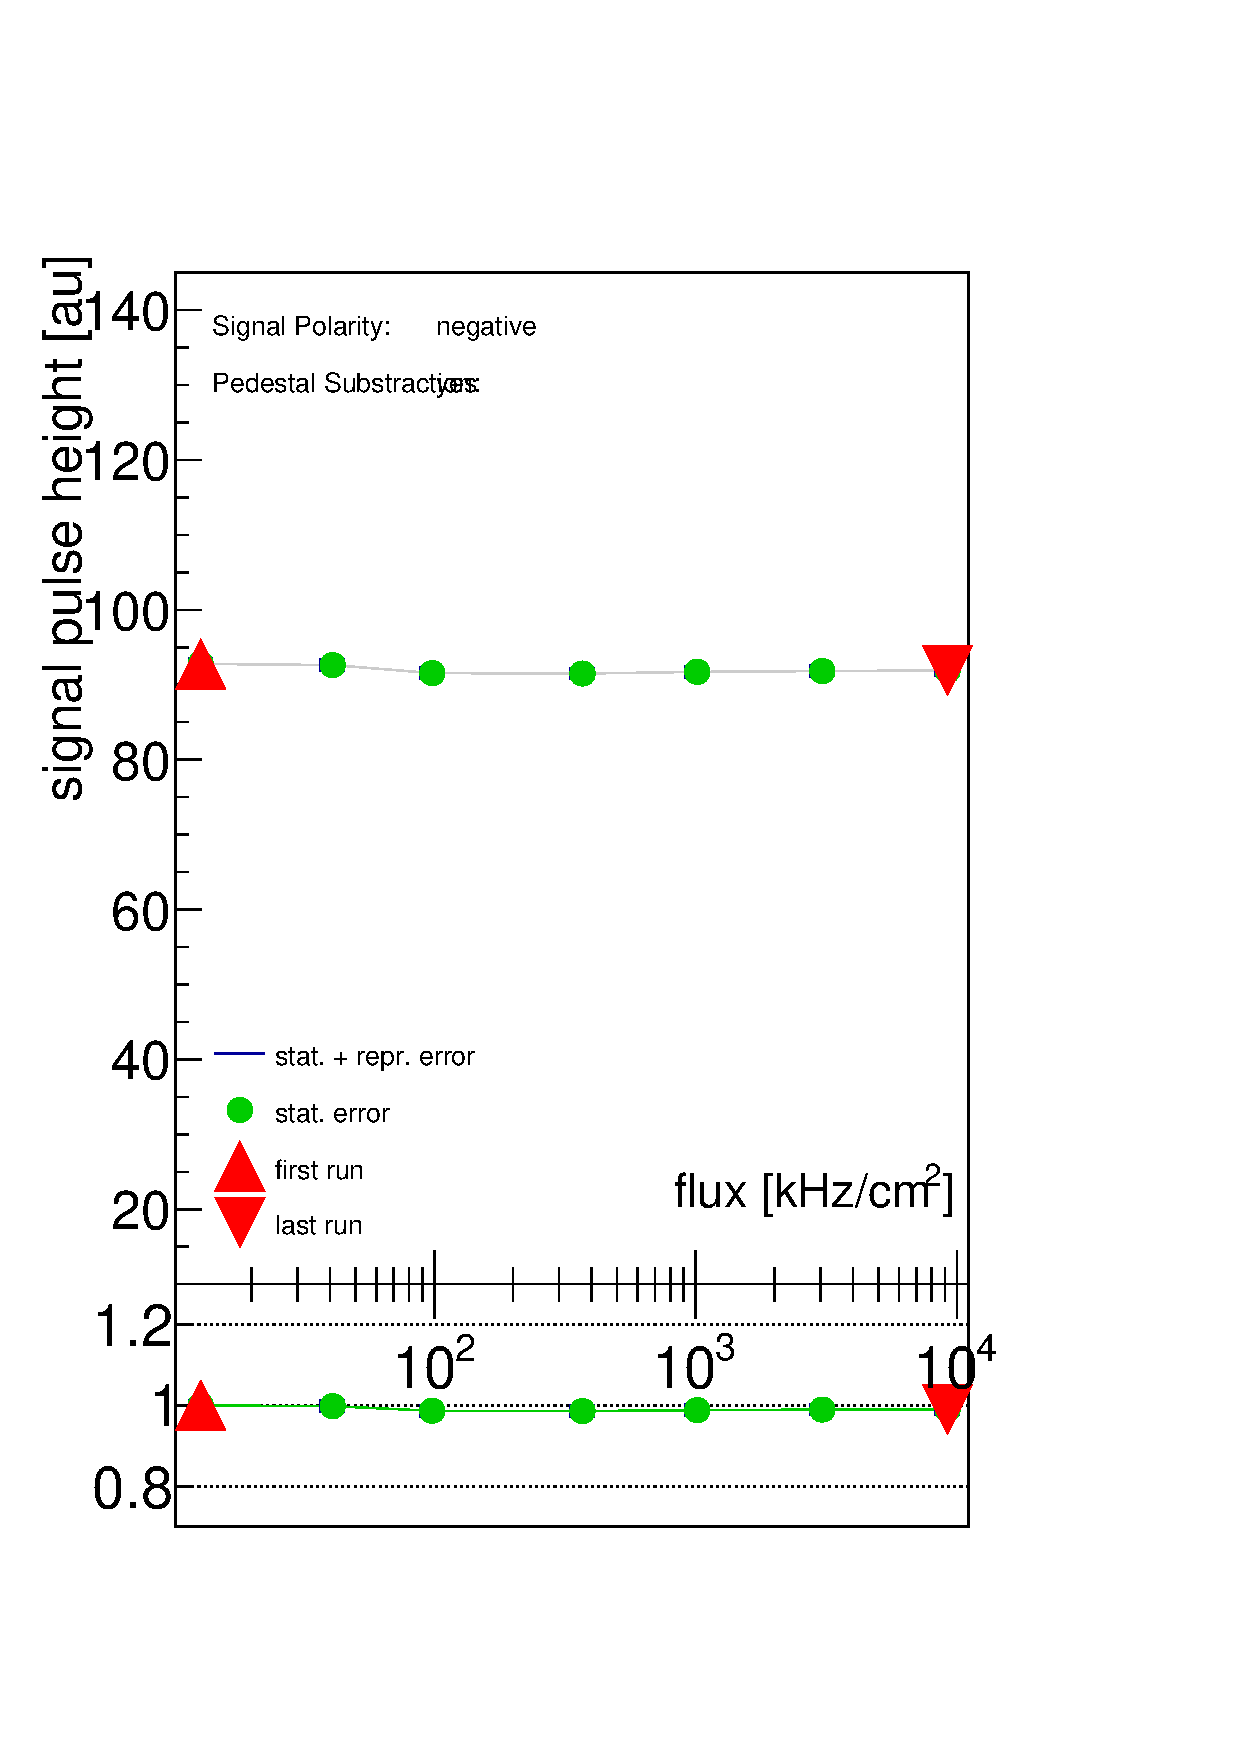
\includegraphics[width=3cm]{CPH1510_08_2.pdf}\\
		noise $\upsigma\approx$ \SI{4.9}{au}
	\end{minipage}
	\hspace*{2pt}
	\begin{minipage}{2.8cm}
		\centering
		August 2016 - \SI[exponent-product = \cdot]{1e15}{n/cm^{2}}
		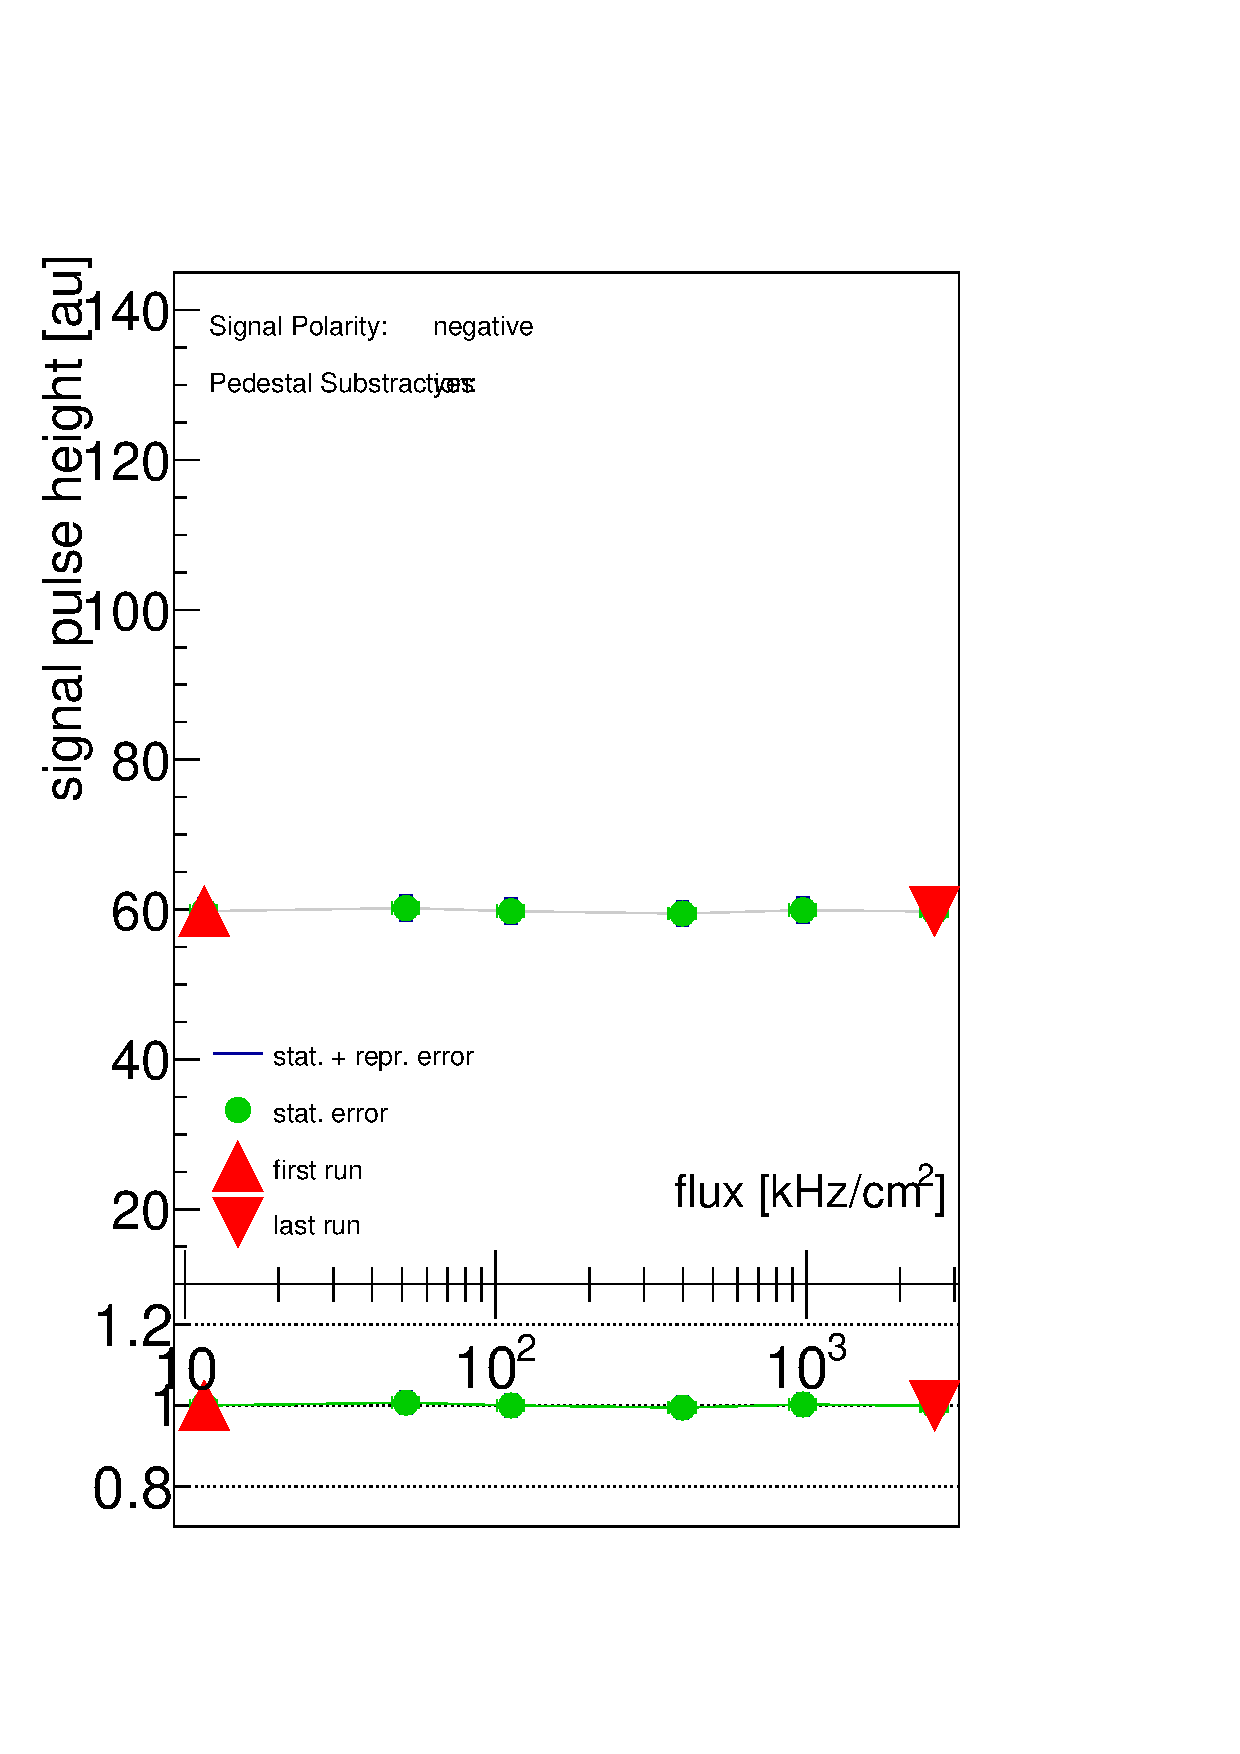
\includegraphics[width=3cm]{CPH1608_09_1.pdf}\\
		noise $\upsigma \approx$ \SI{4.9}{au}
	\end{minipage}
	\hspace*{2pt}
	\begin{minipage}{2.8cm}
		\centering
		October 2016 - \SI[exponent-product = \cdot]{2e15}{n/cm^{2}}
		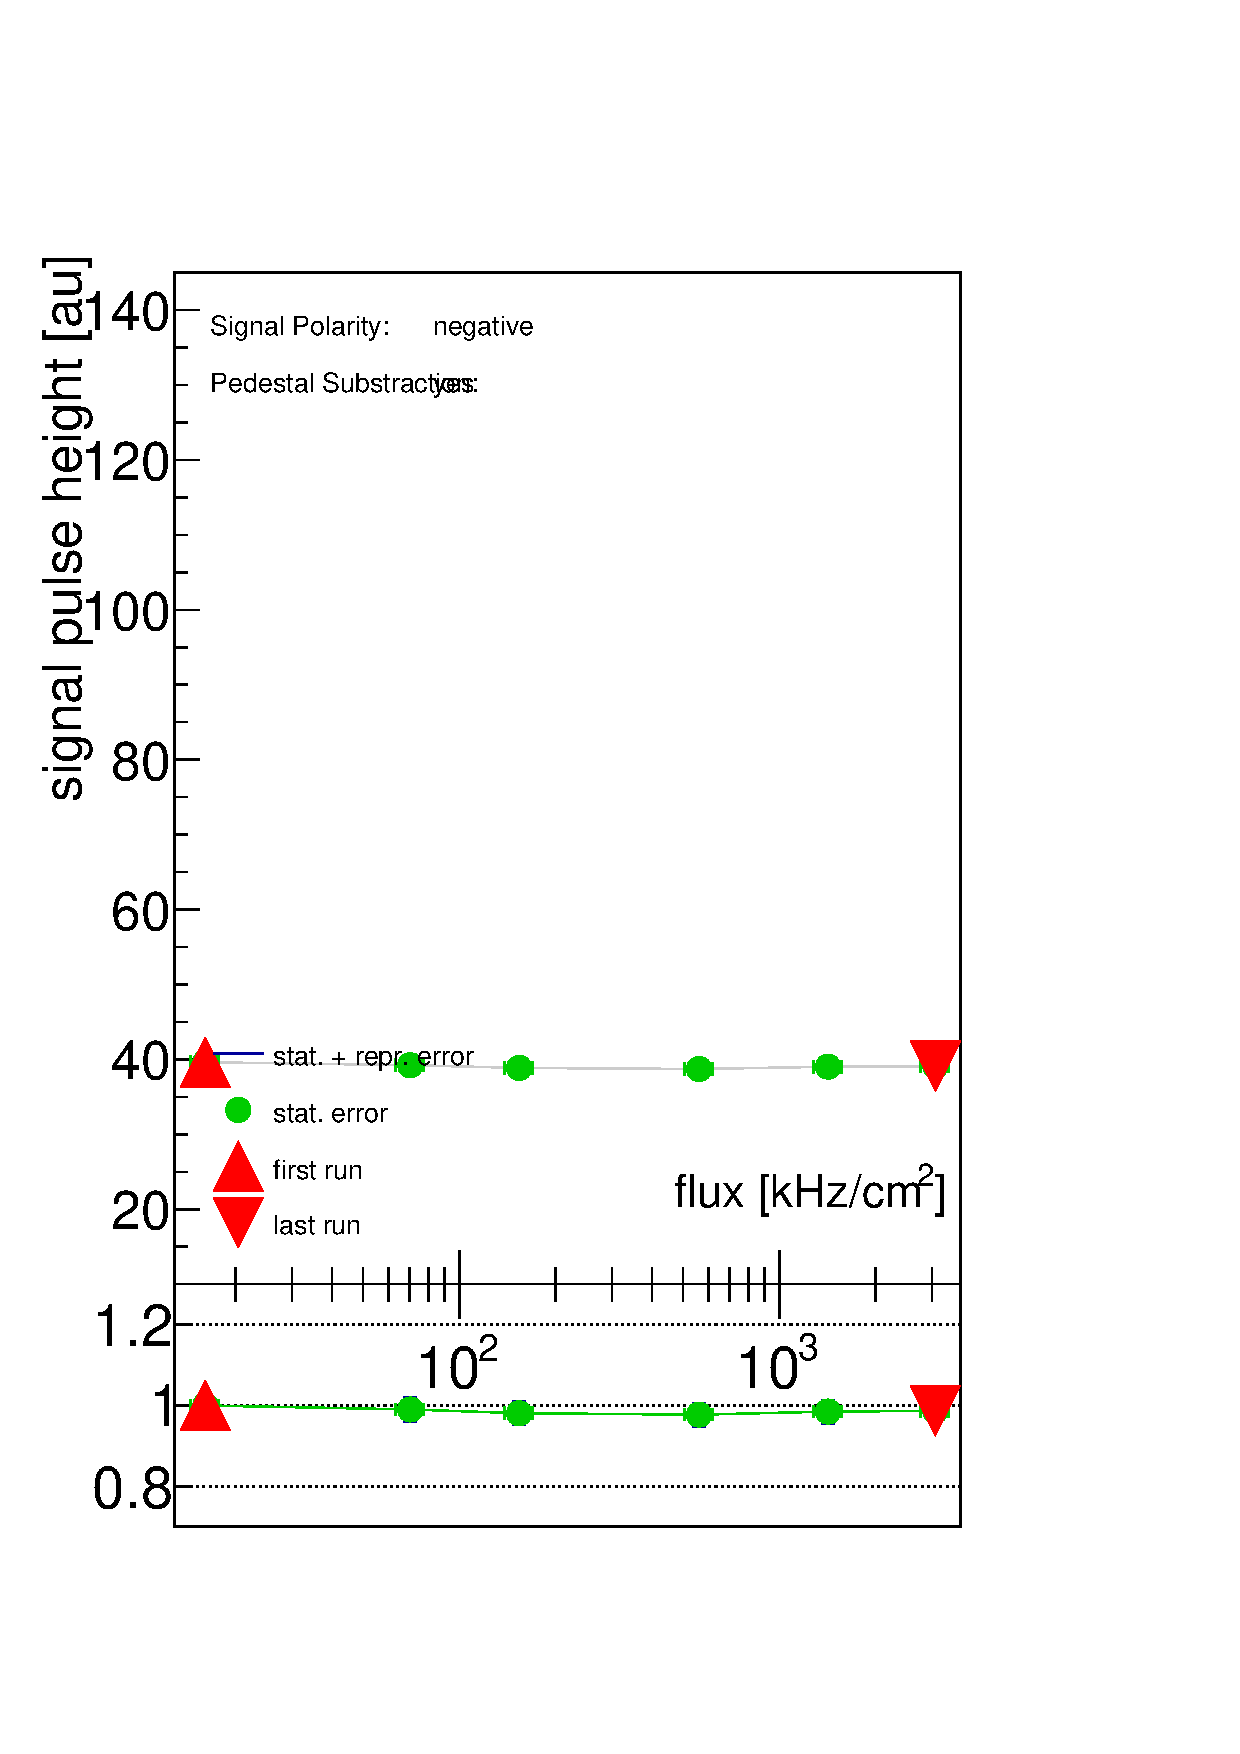
\includegraphics[width=3cm]{CPH1610_6_1.pdf}\\
		noise $\upsigma \approx$ \SI{4.9}{au}
	\end{minipage}\s
	\begin{itemize}
		\item pulse height very stable after irradiation
		\item noise stays the same
	\end{itemize}
\end{frame}
